\clearpage
\subsection{EZ-PICARD - Microservices Practices}

% add image here
\begin{figure}[h]
    \centering
    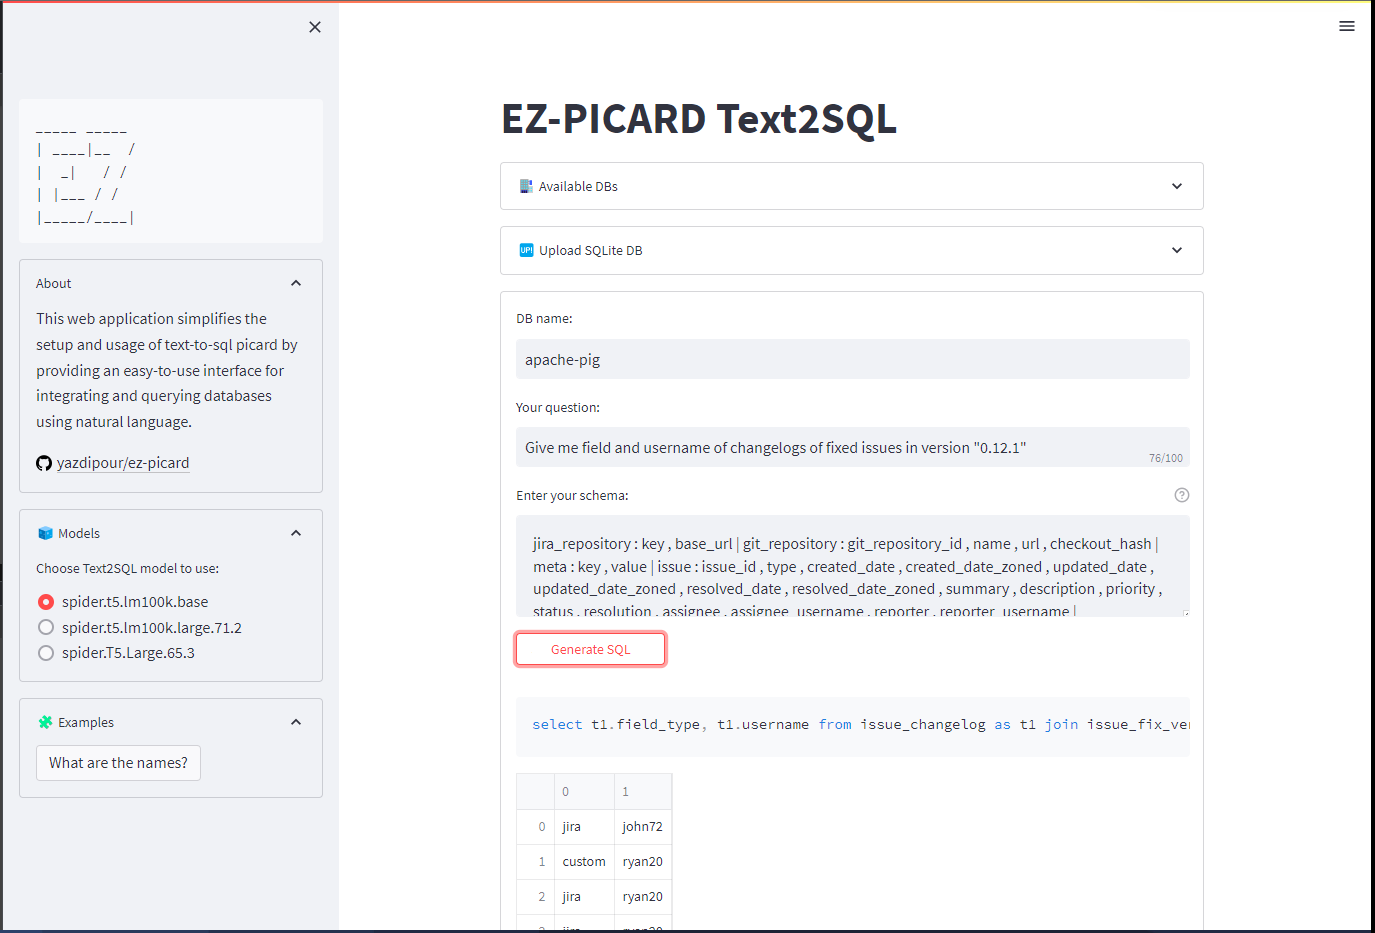
\includegraphics[width=1\textwidth]{pics/ez/ui.png}
    \caption{EZ-PICARD Web Application}
    \label{fig:ezpicard}
\end{figure}

For software engineering practices and to make PICARD setup easier for engineers, researchers, and users, a microservice web service with a web application has been created and open-sourced to the community\footnote[1]{Link to the Github Page: \url{https://github.com/yazdipour/ez-picard/}}. This application consists of a web user interface that gives users the ability to upload their databases and enter their natural language questions and receive queries from our model with values from the database if available. Additionally, a REST API exists for further expansion and usage within the application, providing users with a more versatile and powerful tool for their needs. This web service and application is designed to make the usage of PICARD easier and more accessible for everyone and to allow for the development of new applications and services that utilize its powerful capabilities.

PICARD is a method for constrained inference on top of an existing model, but it is not a model itself. Currently, the PICARD parser and the supporting software are not supported for PostgreSQL, MySQL and others, which would require changes to the PICARD parser, translation of Spider databases and text-to-SQL data, and retraining models to produce MSSQL code. To use the Picard Method, a complex toolchain of Haskell code is built with CABAL and requires a complicated toolchain for the Facebook Thrift library.

% After the setup, the Picard server can be started by running the compiled standalone executable PICARD. This executable is responsible for providing the necessary information to the user, such as specific parameters and options within the constrained inference.

The thrift library is used for communication between the parser and the beam search algorithm. The parser, written in the efficient and powerful Haskell programming language, is used in combination with the hf transformers, which is a Python package. To further expand the scope of the system, new SQL engines can be supported by adding a parser for each one.

These parsers also need to be written in Haskell, as the existing SQLite parser is of limited use in this regard, as it has been written to work best on Spider's subset of SQLite and only supports part of the SQLite specification. This means that more advanced parsers must be created to maximize the system's capabilities. Additionally, these parsers need to be written with a high level of precision in order to ensure that the system can effectively communicate with various engines and databases.

With EZ-PICARD, we can have an adapter layer between SQLite DB and any other database engine, such as MySQL. This layer can be implemented independently from PICARD itself using Python instead of Haskell and can provide a wide range of features, such as automatically translating queries from SQLite to the target database engine and mirroring the schema to the SQLite DB. This adapter layer can provide further advantages by allowing developers to use the same codebase to support multiple database engines, thus reducing the need for additional development and maintenance costs.

% add image here
\begin{figure}[h]
    \centering
    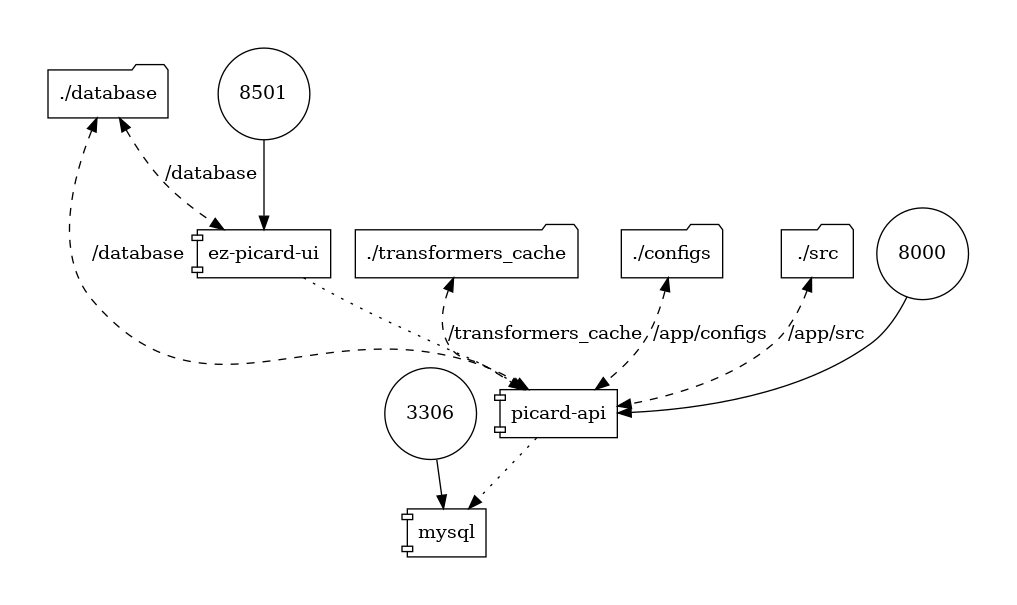
\includegraphics[width=0.8\textwidth]{pics/ez/map.png}
    \caption{EZ-PICARD Architecture}
\end{figure}
